\documentclass[11pt]{article}
\usepackage{geometry}                
\geometry{letterpaper}                   

\usepackage{graphicx}
\usepackage{amssymb}
\usepackage[outdir=./]{epstopdf}
\usepackage{natbib}
\usepackage{amssymb, amsmath}
\usepackage{algorithm, algpseudocode}
\usepackage{caption}
\usepackage{subcaption}
\usepackage{pdfpages}

\DeclareGraphicsRule{.tif}{png}{.png}{`convert #1 `dirname #1`/`basename #1 .tif`.png}

%\title{Title}
%\author{Name 1, Name 2}
%\date{date} 

\begin{document}



\thispagestyle{empty}

\begin{center}
\includegraphics[width=5cm]{ETHlogo.eps}

\bigskip


\bigskip


\bigskip


\LARGE{ 	Lecture with Computer Exercises:\\ }
\LARGE{ Modelling and Simulating Social Systems with MATLAB\\}

\bigskip

\bigskip

\small{Project Report}\\

\bigskip

\bigskip

\bigskip

\bigskip


\begin{tabular}{|c|}
\hline
\\
\textbf{\LARGE{Influence of Success-Driven and Reputation-Based}}\\
\textbf{\LARGE{Migration in the Evolution of Cooperation}}\\
\\
\hline
\end{tabular}
\bigskip

\bigskip

\bigskip

\LARGE{Byungsoo Kim \& Basile Maret}



\bigskip

\bigskip

\bigskip

\bigskip

\bigskip

\bigskip

\bigskip

\bigskip

Zurich\\
December 2015\\

\end{center}



\newpage

%%%%%%%%%%%%%%%%%%%%%%%%%%%%%%%%%%%%%%%%%%%%%%%%%

\newpage
\section*{Agreement for free-download}
\bigskip


\bigskip


\large We hereby agree to make our source code for this project freely available for download from the web pages of the SOMS chair. Furthermore, we assure that all source code is written by ourselves and is not violating any copyright restrictions.

\begin{center}

\bigskip


\bigskip


\begin{tabular}{@{}p{3.3cm}@{}p{6cm}@{}@{}p{6cm}@{}}
\begin{minipage}{3cm}

\end{minipage}
&
\begin{minipage}{6cm}
\vspace{2mm} \large Byungsoo Kim

 \vspace{\baselineskip}

\end{minipage}
&
\begin{minipage}{6cm}

\large Basile Maret

\end{minipage}
\end{tabular}


\end{center}
\newpage

%%%%%%%%%%%%%%%%%%%%%%%%%%%%%%%%%%%%%%%



% IMPORTANT
% you MUST include the ETH declaration of originality here; it is available for download on the course website or at http://www.ethz.ch/faculty/exams/plagiarism/index_EN; it can be printed as pdf and should be filled out in handwriting
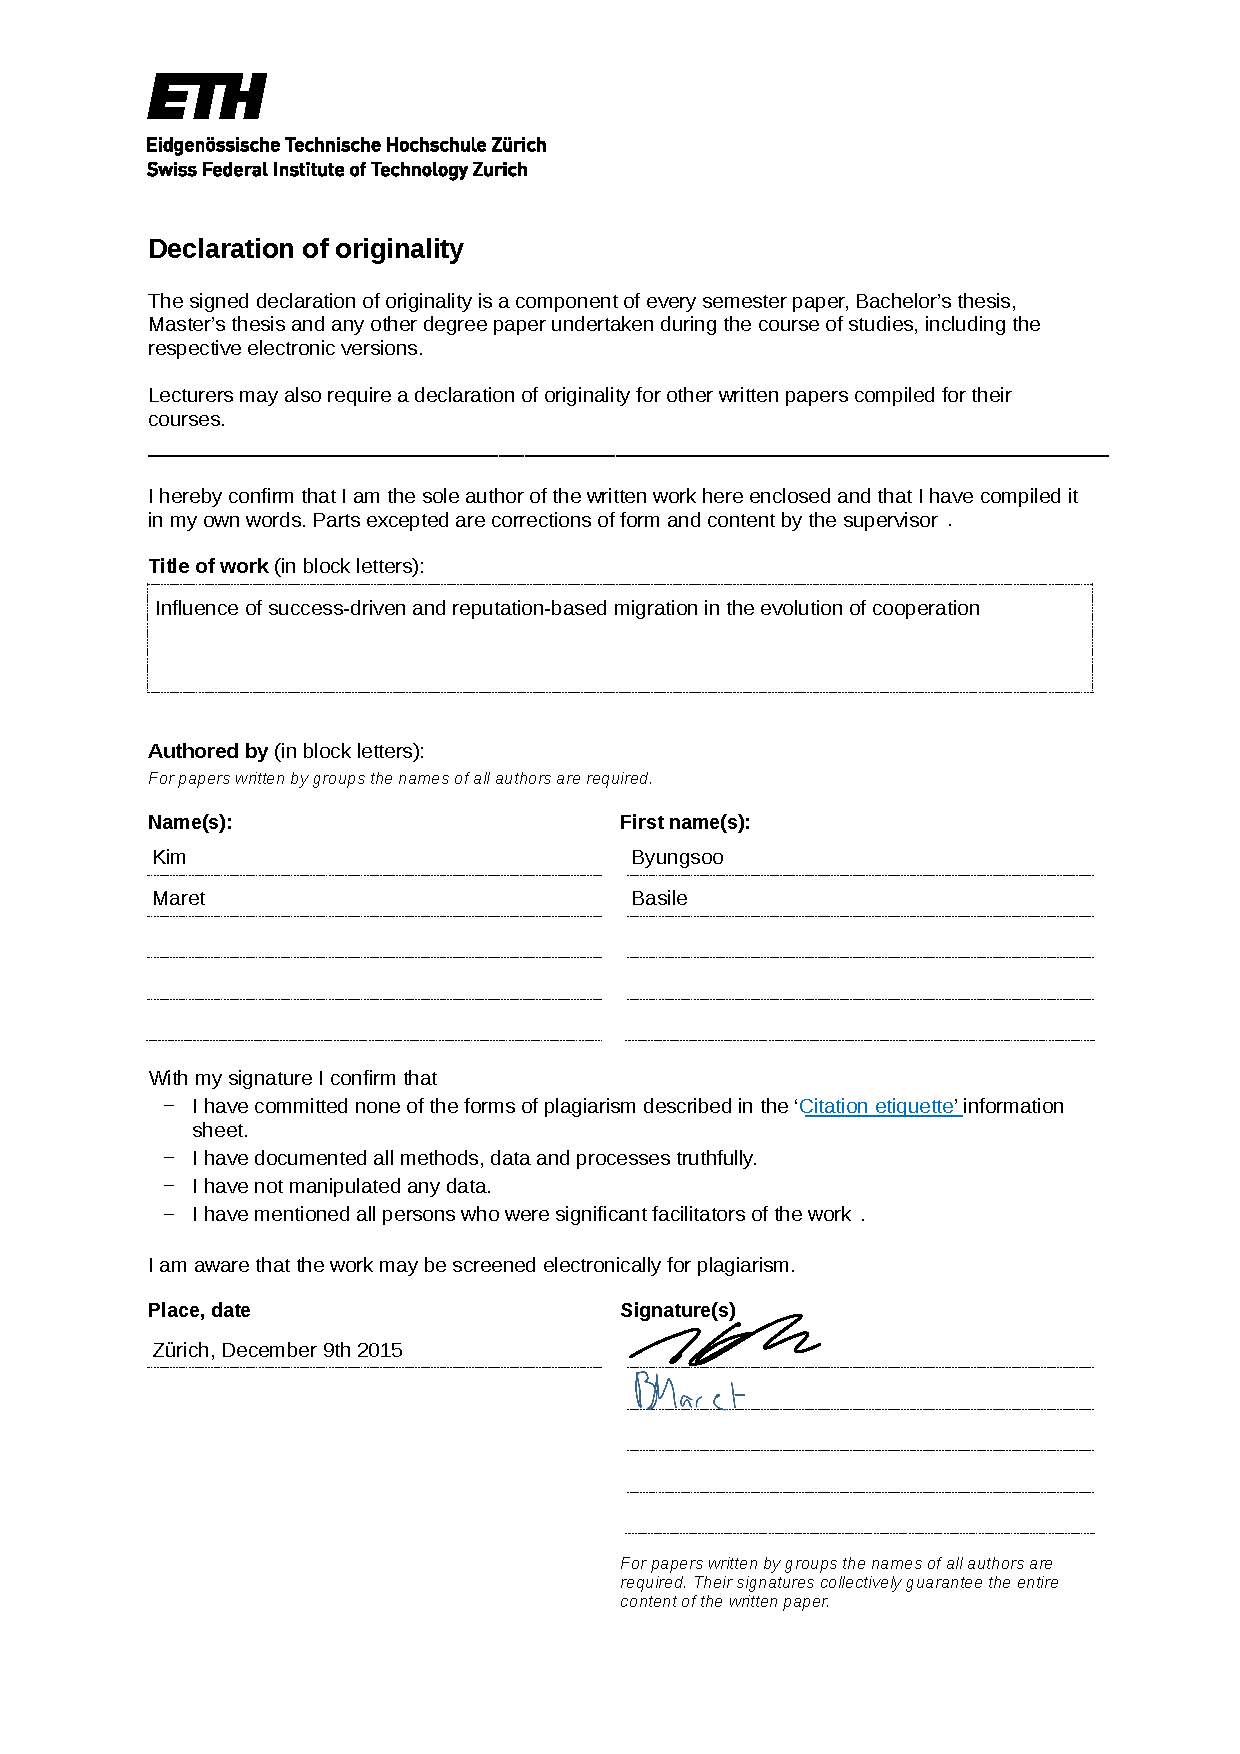
\includepdf[pages=-]{../declaration-originality.pdf}



%%%%%%%%%% Table of content %%%%%%%%%%%%%%%%%

\tableofcontents

\newpage

%%%%%%%%%%%%%%%%%%%%%%%%%%%%%%%%%%%%%%%



\section{Abstract}
Cooperation is one of the most important issue in the society in terms of the stability and productivity of the society where individuals pursue selfishness. Many studies have tried to explain the evolution of cooperation among unrelated individuals, and we can improve our understanding about it in a game-theoretical way. Most of the time, in real life, more than one factor play a role at the same time. Our model in this paper is designed to reflect that fact. It is the combination of the success-driven and reputation-based migration model to decide where to go and whether move or not \textit{simultaneously}. As a result of comparison with existing models, our model shows that it is distinguishable from the reputation-based migration model in terms of convergence, cooperator ratios and cooperator patterns by getting the predictability of the success-driven migration model. Compared to the success-driven migration model, it gets cooperator ratio as high as the one from the success-driven migration model with a more natural way of migrating.

\section{Individual contributions}
\subsection{Byungsoo Kim}
\begin{itemize}
\item Implementation of the Success-Driven Migration Model
\item Implementation of the Reputation-Based Migration Model
\item Analysis of the Models
\item Redaction of the report
\end{itemize}

\subsection{Basile Maret}
\begin{itemize}
\item Experiment of the Success-Driven Migration Model
\item Experiment of the Reputation-Based Migration Model
\item Analysis of the Models
\item Redaction of the report
\end{itemize}

\newpage
\section{Introduction and Motivations}

Cooperation is one of the most important issue in the society in terms of the stability and productivity of the society where individuals pursue selfishness. Many studies have tried to explain the evolution of cooperation among unrelated individuals, and we can improve our understanding about it in a game-theoretical way. Individuals are affected by interacting with neighbours so that their life is affected in either positive or negative way. Through the interaction, they notice the relative situation of their life and take an action to improve it. For instance, \textit{imitation} of neighbour's superior strategy (be cooperator or defector) or \textit{migration} to some other place which has a better potential benefit. There are existing models for each action.

In the \textit{success-driven} migration model [1][2], it assumes that individuals prefer to migrate to the place where they can get the best benefit within a certain area. In an empty place, it is possible to estimate the potential benefit based on the assumption that they migrate to there and interact with their neighbours around it. Provided better potential benefit than the one of current place, individuals \textit{immediately move} to the best candidate place.  

On the other hand, individuals can maximize their future benefit by considering the reputation of their neighbours as a long-term plan, not the potential benefit of the empty sites. In the \textit{reputation-based} migration model [3], individuals evaluate their neighbours based on their reputation. As for reputation here, a cooperator has higher reputation than a defector, and it can be accumulated over time. Contrary to the success-driven migration model, individuals \textit{decide whether move or not} based on the neighbours' overall reputation before migrating to a random empty place.

Most of the time, in real life, more than one factor play a role at the same time. Our model in this paper is designed to reflect that fact. It is the combination of the success-driven and reputation-based migration model to decide where to go and whether move or not \textit{simultaneously}. Lastly, we will look in detail how this model will influence the evolution of cooperation.


\section{Description of the Model}
\subsection{Prisoner's Dilemma}

We will use the well known prisoner's dilemma game in a game-theoretical way. In this game, the players can take an action among two options: either cooperate or defect. According to their behaviour, there is a payoff which motivate them to defect mutually rather than cooperate. It is represented by the payoff matrix below:

\begin{figure}[!htbp]
	\centering
	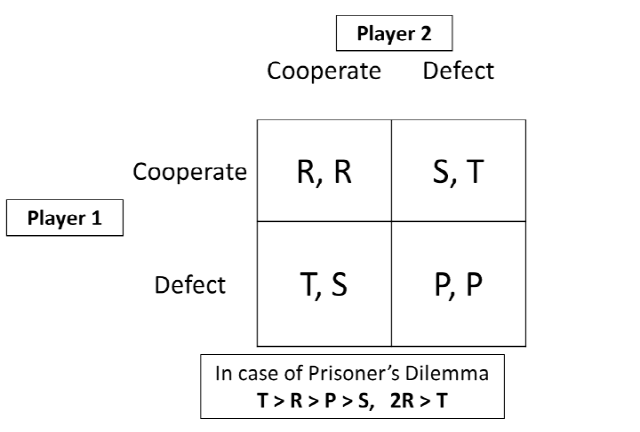
\includegraphics[scale=0.72]{../../other/pd_payoff_matrix.png}
    \caption{Payoff Matrix of Prisoner's Dilemma}
    \label{fig:paymatrix}
\end{figure}

\newpage
As shown in figure~\ref{fig:paymatrix}, mutual cooperation gives reward payoff $R$ to both players. One defection between two players gives the temptation payoff $T$ for defector which is larger than $R$ so that it induces the player to defect when the opponent cooperates. The opponent will get what is called the sucker's payoff $S$. In case of mutual defection, they will get punishment $P$ payoff which is larger than $S$ so that it also induces the player to defect when the opponent defect. In sum, everybody is expected to defect, called the \textit{"tragedy of the commons"} (Hardin, 1968). We used a simplified version of the prisoner's dilemma game by setting $T=b$, $R=1$, $P=S=0$ [3]. 


\subsection{Spatial Game with Strategies}

We simply model social interactions on the $L \times L$ 2-dimensional spatial grid [1]. There are $N$ individuals occupying grid sites with the ratio $\rho$, and they interact with $m$ direct neighbours (von Neumann neighbourhoods). The overall payoff $P$ of player $i$ at iteration $t$ is the sum of each payoffs resulting from binary interactions with all von Neumann neighbours [2], and the respective player "imitate" the strategy of best performing neighbour.

In addition, we will extend this game by including both success-driven migration and reputation-based migration. Before the imitation step, a player can move to improve their expected overall payoff to empty site within a quadratic area of $(2M+1) \times (2M+1)$ sites (the Moore neighbourhood of size $M$, e.g. the 8 neighbouring sites for $M = 1$). A player can also evaluate the surrounding environment and decide whether he leaves or not by comparing his reputation and those of his neighbours [3]. Below equations account for the reputation effect in mobility:

\begin{figure}[!htbp]
	\centering
	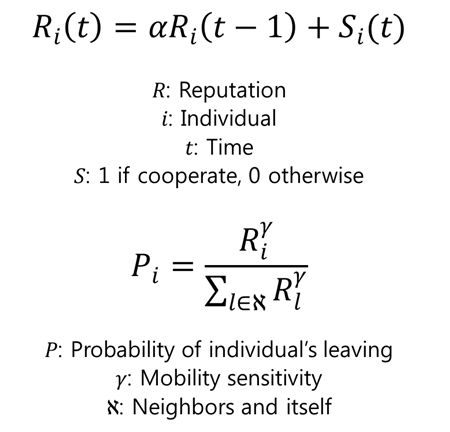
\includegraphics[scale=0.7]{../../other/reputation_eq.png}
    \caption{Reputation Equations}
    \label{fig:reputationeq}
\end{figure}



\section{Implementation}
The code for each model is implemented in \verb|code/cooperation.m|, and the code for the experiment is implemented in \verb|code/cooperation_script.m|. The initial population density $\rho$ is 0.7, and the ration of the cooperators to the defectors is 0.5.

\subsection{Strategy Imitation}
Basically, all models include \verb|Strategy Imitation| procedure as follows:

\begin{algorithm}[H]
  \caption{Strategy Imitation}\label{imitation}
  \begin{algorithmic}[1]
    \Procedure{Strategy Imitation}{$r,c$}
      \State $payoff_{max} \gets payoff_{r,c}$
      \State $r_{max},c_{max} \gets r,c$
      \For{$neighbour \gets neighbours$}\Comment{von Neumann Neighbour $m$}
      	\If {$payoff_{neighbour} > payoff_{max}$}\Comment{Find the Best Neighbour}
        \State $payoff_{max} \gets payoff_{neighbour}$
        \State $r_{max},c_{max} \gets r_{neighbour},c_{neighbour}$
        \EndIf
      \EndFor
      \State $strategy_{r,c} \gets strategy_{r_{max},c_{max}}$   \Comment{Imitate Strategy (Cooperator or Defector)}
    \EndProcedure
  \end{algorithmic}
\end{algorithm}


\subsection{Success-Driven Migration Model}
In success-driven migration model, each individual update its payoff and compute the fictitious payoff of empty neighbour sites, then migrate to there as follows:

\begin{algorithm}[H]
  \caption{Success-Driven Migration Model}\label{successdriven}
	\begin{algorithmic}[1]
	\Procedure{Success-Driven Migration Model}{}
		\For{$iter \gets 1 \textrm{ to } iter_{max}$}
		\For{$r,c \gets grid$}	\Comment{In Random Sequential Order}
			\State \textbf{Update Payoff$(r,c)$}
			\State $r_{new},c_{new} \gets$ \textbf{Success-Driven Migration$(r,c)$}
			\State \textbf{Strategy Imitation$(r_{new},c_{new})$}
		\EndFor      
		\EndFor      
    \EndProcedure
	\end{algorithmic}
		
	\begin{algorithmic}[1]
    \Procedure{Update Payoff}{$r,c$}
      \For{$neighbour \gets neighbours$}\Comment{von Neumann Neighbour $m$}
      	\State $payoff_{r,c} \gets payoff_{r,c} + payoffMatrix(r,c, neighbour)$ \Comment{Matrix of $T,R,P,S$}
      \EndFor      
    \EndProcedure
  \end{algorithmic}		
		
	\begin{algorithmic}[1]
    \Procedure{Success-Driven Migration}{$r,c$}
      \State $payoff_{max} \gets payoff_{r,c}$\Comment{The Maximum Fictitious Payoff}
      \State $r_{max},c_{max} \gets r,c$
      \For{$neighbour \gets neighbours$}\Comment{Empty Sites in Moore Neighbour $M$}
      	\If {$payoff_{neighbour} > payoff_{max}$}\Comment{Find the Best Neighbour}
        \State $payoff_{max} \gets payoff_{neighbour}$
        \State $r_{max},c_{max} \gets r_{neighbour},c_{neighbour}$
        \EndIf
      \EndFor
      \State $strategy_{r_{max},c_{max}} \gets strategy_{r,c}$   \Comment{Migrate to the Best Candidate}
      \State $payoff_{r_{max},c_{max}} \gets payoff_{r,c}$
      \State $strategy_{r,c} \gets empty$   \Comment{Make Previous Site Clear}
      \State $payoff_{r,c} \gets 0$
      \State \textbf{return} $r_{new},c_{new}$	\Comment{Return Migrated Site}
    \EndProcedure
  \end{algorithmic}
\end{algorithm}


\subsection{Reputation-Based Migration Model}
In reputation-based migration model, individuals compute the reputation of neighbours and leaving probability based on it. Then, move to a random empty site and imitate strategy as follows:

\begin{algorithm}[H]
  \caption{Reputation-Based Migration Model}\label{reputationbased}
	\begin{algorithmic}[1]
	\Procedure{Reputation-Based Migration Model}{}
		\For{$iter \gets 1 \textrm{ to } iter_{max}$}
		\For{$r,c \gets grid$}	\Comment{Random order}
			\State \textbf{Update Payoff$(r,c)$}
			\State {$P \gets$ \textbf{Compute Reputation$(r,c,\gamma,\alpha)$}}
			\State $r_{new},c_{new} \gets$ \textbf{Random Migration$(r,c,P)$}
			\State \textbf{Strategy Imitation$(r_{new},c_{new})$}
		\EndFor      
		\EndFor      
    \EndProcedure
	\end{algorithmic}
\end{algorithm}

\begin{algorithm}[H]
  \caption{Reputation-Based Migration}\label{reputationbasedmigration}
	\begin{algorithmic}[1]
    \Procedure{Compute Reputation}{$r,c,\gamma,\alpha$}
      \State $sum_{reputation} \gets 0$\Comment{Sum of Neighbours Reputation}
	  \State $P \gets 0$\Comment{The Probability of Leaving}
      \For{$neighbour \gets neighbours$}\Comment{Empty Sites in Moore Neighbour $M$}
        \State $sum_{reputation} \gets sum_{reputation} + reputation_{neighbour}^{\gamma}$
      \EndFor
      \If {$sum_{reputation} > 0$}
      	\State $P \gets reputation_{r,c}^{\gamma} / sum_{reputation}$
      \EndIf
      \State $reputation_{r,c} \gets reputation_{r,c} \times \alpha$ \Comment{Update Own reputation}
      \If {$strategy_{reputation} == cooperator$ }
      	\State $reputation_{r,c} \gets reputation_{r,c} + 1$
      \EndIf
      \State \textbf{return} $P$ \Comment{Return the Probability of Leaving}
    \EndProcedure
  \end{algorithmic}
		
	\begin{algorithmic}[1]
    \Procedure{Random Migration}{$r,c,P$}
      \State{$neighbour \gets rand(neighbours,P)$} \Comment{Select an Empty Sites in Moore Neighbour $M$}
      \State $strategy_{r_{neighbour},c_{neighbour}} \gets strategy_{r,c}$   \Comment{Migrate to the Neighbour}
      \State $payoff_{r_{neighbour},c_{neighbour}} \gets payoff_{r,c}$
      \State $strategy_{r,c} \gets empty$   \Comment{Make Clear Previous Site}
      \State $payoff_{r,c} \gets 0$
      \State \textbf{return} $r_{new},c_{new}$	\Comment{Return Migrated Site}
    \EndProcedure
  \end{algorithmic}
\end{algorithm}


\subsection{Our Model}
Our model, which is the combination of success-driven migration and reputation-based migration model, is in the following:

\begin{algorithm}[H]
  \caption{Success-Driven and Reputation-Based Migration Model}\label{ourmodel}
	\begin{algorithmic}[1]
	\Procedure{Success-Driven and Reputation-Based Migration Model}{}
		\For{$iter \gets 1 \textrm{ to } iter_{max}$}
		\For{$r,c \gets grid$}	\Comment{Random order}
			\State \textbf{Update Payoff$(r,c)$}
			\State $P \gets$ \textbf{Compute Reputation$(r,c,\gamma,\alpha)$}
			\State $r_{new},c_{new} \gets r,c$
			\If {$P > rand()$}	\Comment{with the Probability of Leaving}
				\State $r_{new},c_{new} \gets$ \textbf{Success-Driven Migration$(r,c)$}
			\EndIf
			\State \textbf{Strategy Imitation$(r_{new},c_{new})$}
		\EndFor      
		\EndFor      
    \EndProcedure
	\end{algorithmic}
\end{algorithm}

\subsection{Other models}
To look at the migration patterns, we used three more models :
\begin{enumerate}
\item Success-Driven migration without imitation
\item Reputation-Based migration without imitation
\item Success-Driven and Reputation-Based migration without imitation
\end{enumerate}

These models don't really represent real life situations but we used them compare how the different migrations work without the effect of imitation.

\newpage
\section{Simulation Results and Discussion}
In this section, we present the results of our simulations. 

\subsection{Convergence}
It is easy to see on the plots that the success-driven migration model, the model with imitation only and our model converge to a stable cooperator ratio in less than 5000 iterations. This was the case for all the different parameters $\alpha$ and $\gamma$ that we tried.
The success-driven migration model always converges faster than our model. This is because our model has a smaller rate of migration.
\begin{figure}[!h]
	\centering
        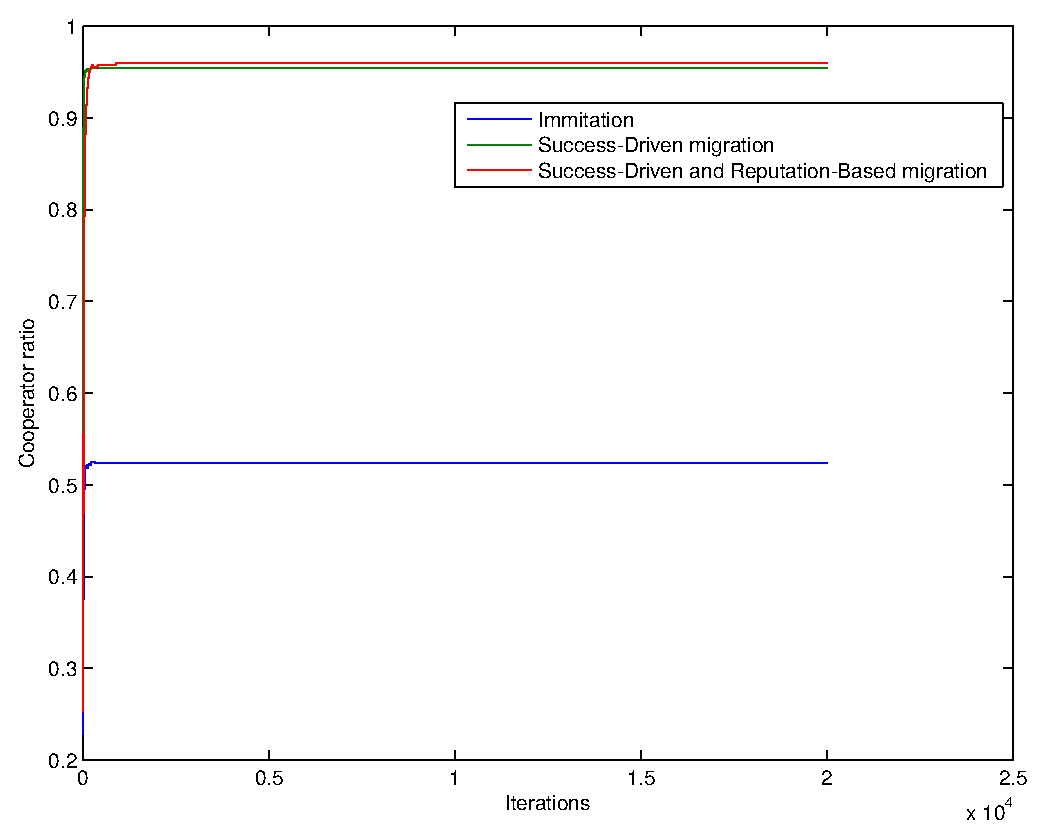
\includegraphics[width=0.5\textwidth]{../../other/plots/convergence-20000.eps}
	\caption{Cooperator ratios after a big number of iterations. We can see that the three models converge in about 2000 iterations. We used the parameters $\alpha = 0.5$ and $\gamma = 500$}
\end{figure}

\begin{figure}
	\centering
	\begin{subfigure}[t]{0.4\textwidth}
        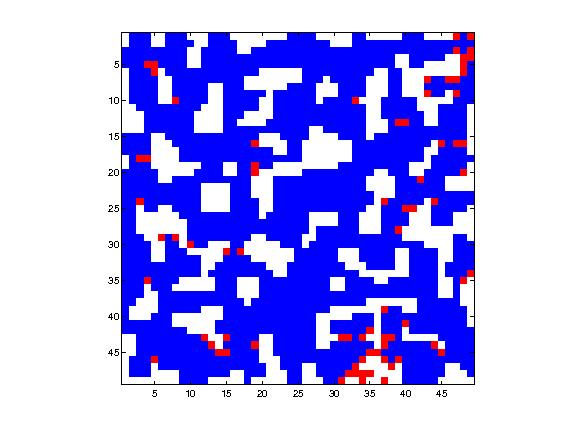
\includegraphics[width=\textwidth]{../../other/grids/m2-t1000.jpg}
	\caption{Grid after 1000 iterations}
    	\end{subfigure}
	\begin{subfigure}[t]{0.4\textwidth}
        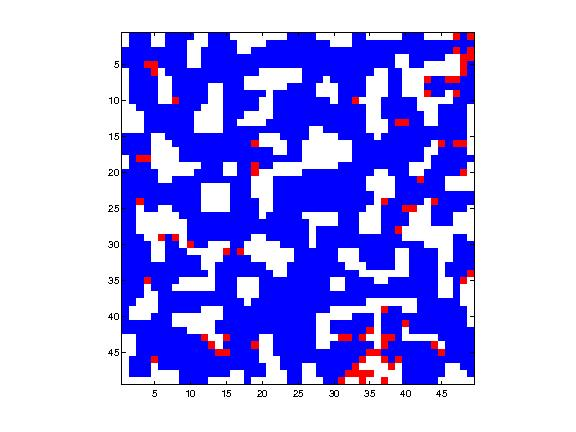
\includegraphics[width=\textwidth]{../../other/grids/m2-t3000.jpg}
	\caption{Grid after 3000 iterations}
    	\end{subfigure}

	\caption{Grids for the Success-Driven migration model after different number of iterations. We can see that it almost doesn't change and reached a stable state.}
	\label{fig:grids_stable}
\end{figure}

\begin{figure}
	\centering
	\begin{subfigure}[t]{0.4\textwidth}
        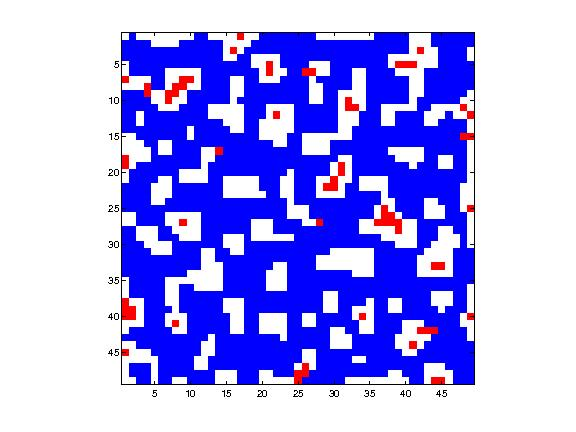
\includegraphics[width=\textwidth]{../../other/grids/m6-t1000.jpg}
	\caption{Grid after 1000 iterations}
    	\end{subfigure}
	\begin{subfigure}[t]{0.4\textwidth}
        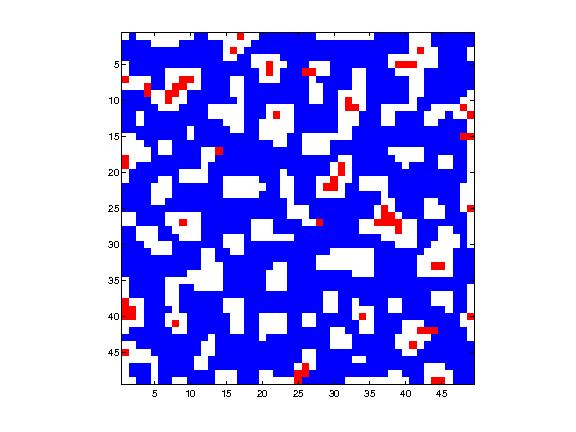
\includegraphics[width=\textwidth]{../../other/grids/m6-t3000.jpg}
	\caption{Grid after 3000 iterations}
    	\end{subfigure}

	\caption{Grids for the Success-Driven and Reputation-Based migration model after different number of iterations. We can see that it almost doesn't change and reached a stable state. We used the parameters $\alpha = 0.5$ and $\gamma = 500$}
	\label{fig:grids_stable}
\end{figure}

The reputation-based migration model only reached a stable cooperator ratio after a number of iteration in the order of 30'000. This is due to the random nature of the migration. The player don't choose an empty place based on their interest to migrate but get assigned a random one. Our simulations didn't have results that could give us certainty that this stable cooperator ratio is always reached and that there won't be an instability after a greater number of iterations.

\begin{figure}
	\centering
	\begin{subfigure}[t]{0.48\textwidth}
        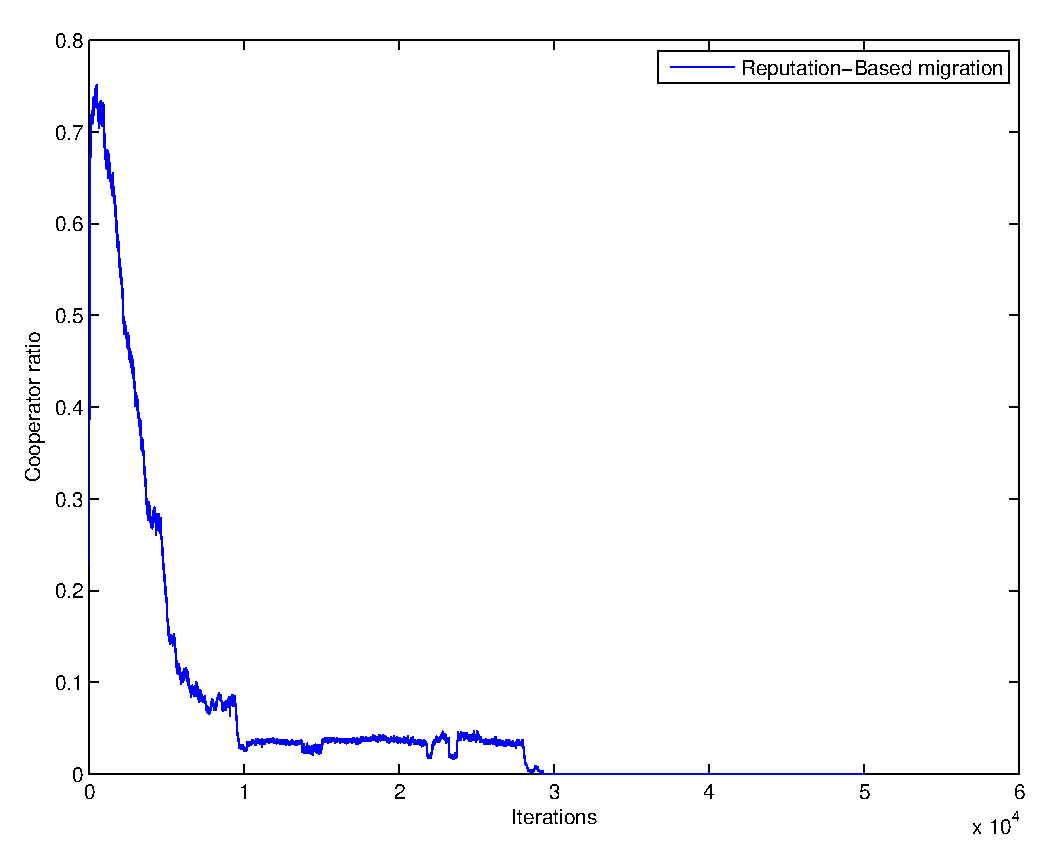
\includegraphics[width=\textwidth]{../../other/plots/convergence-50000.eps}
	\caption{First run}
    	\end{subfigure}
	\begin{subfigure}[t]{0.48\textwidth}
        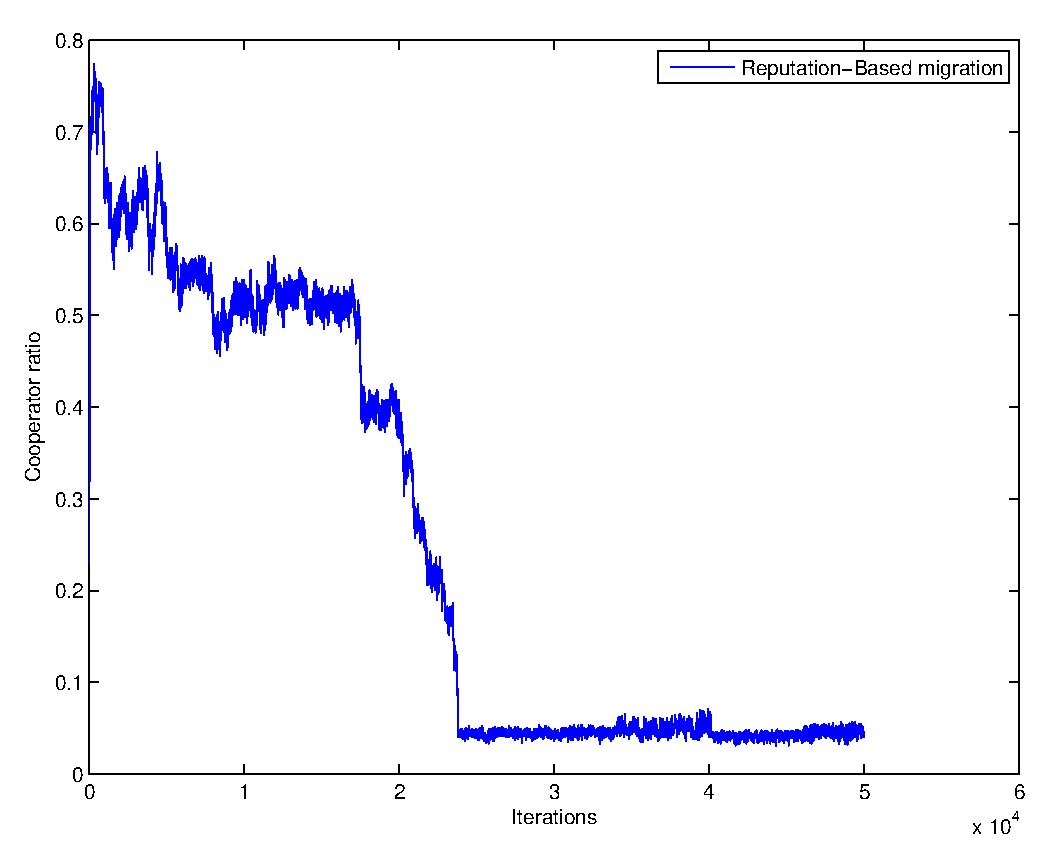
\includegraphics[width=\textwidth]{../../other/plots/convergence-50000-2.eps}
	\caption{Second run}
    	\end{subfigure}

	\caption{Cooperator ratios for Reputation-Based migration. We used the parameters $\alpha = 0.5$ and $\gamma = 500$}
	\label{fig:convergence_reputation}
\end{figure}

\newpage
\subsection{Cooperator ratios}

To compare the cooperator ratios, we plotted the evolution of the ratios over the iterations for different parameters $\gamma$ and $\alpha$.

\begin{figure}
	\centering
	\begin{subfigure}[t]{0.48\textwidth}
        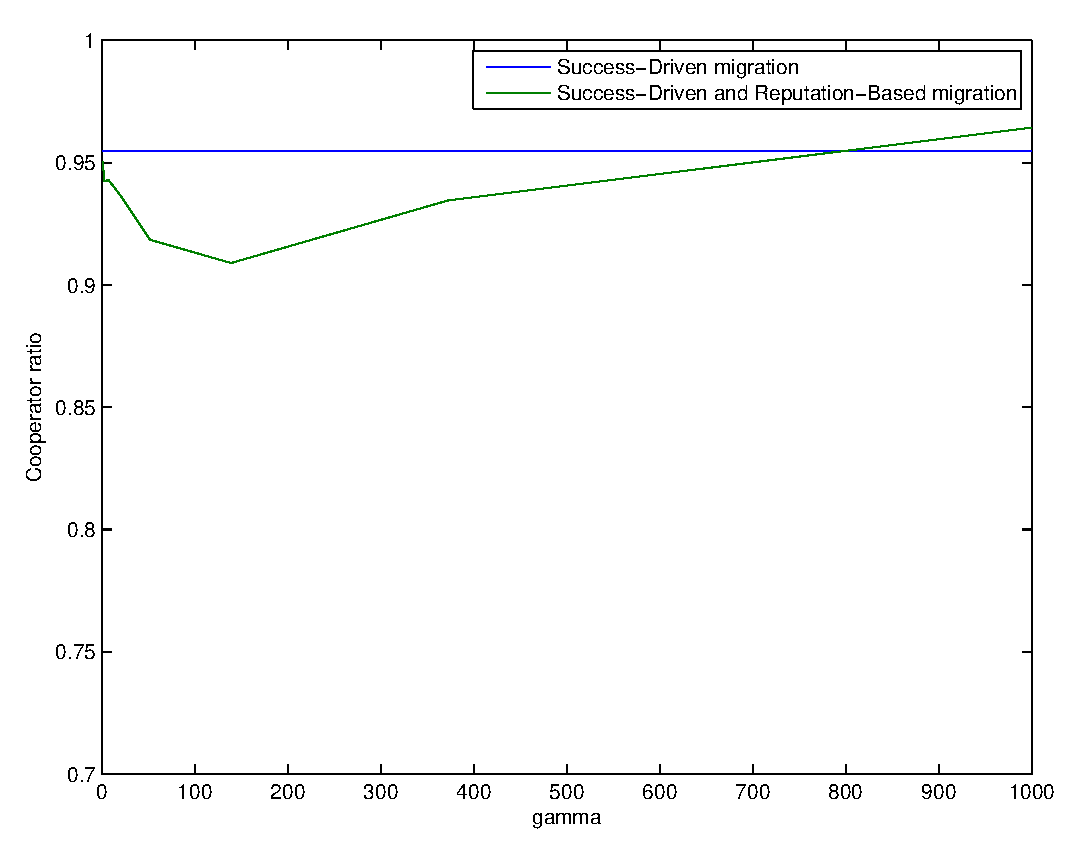
\includegraphics[width=\textwidth]{../../other/plots/alpha01.eps}
	\caption{$\alpha = 0.1$}
	\label{fig:cooperator_ratios_5000-1}
    	\end{subfigure}
	\begin{subfigure}[t]{0.48\textwidth}
        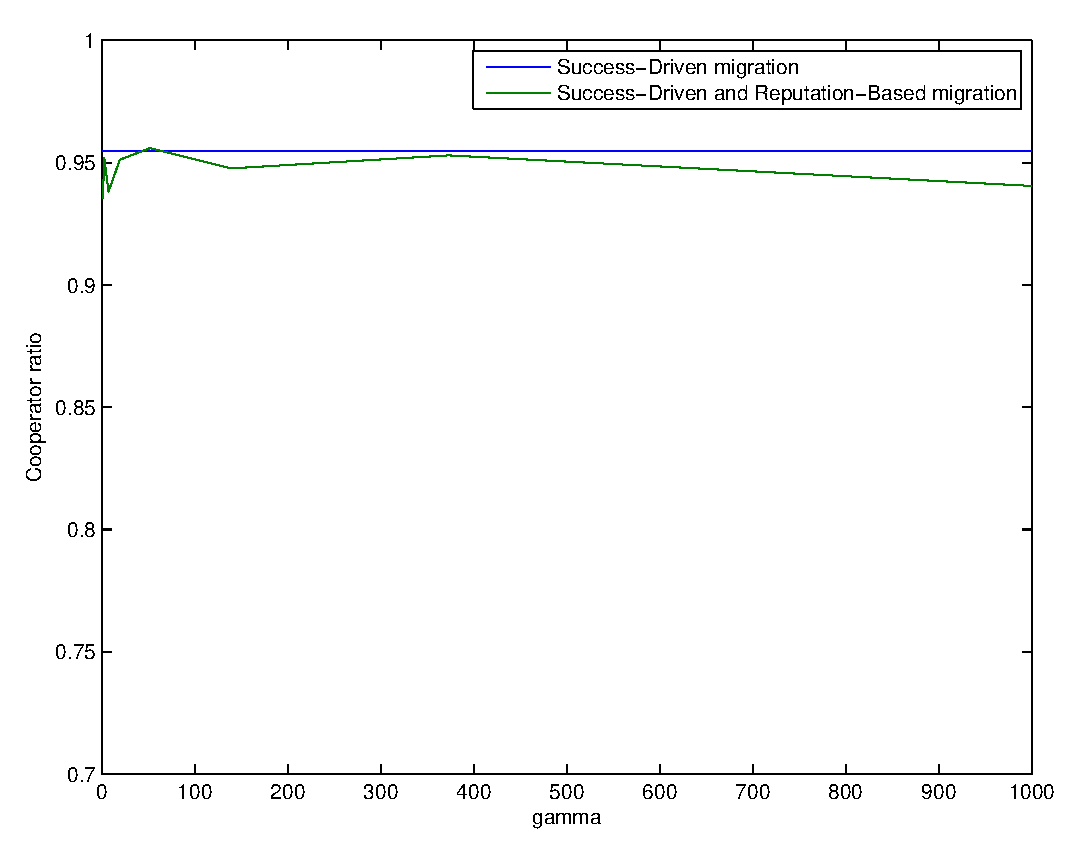
\includegraphics[width=\textwidth]{../../other/plots/alpha05.eps}
	\caption{$\alpha = 0.5$}
	\label{fig:cooperator_ratios_5000-2}
    	\end{subfigure}

	\begin{subfigure}[t]{0.48\textwidth}
        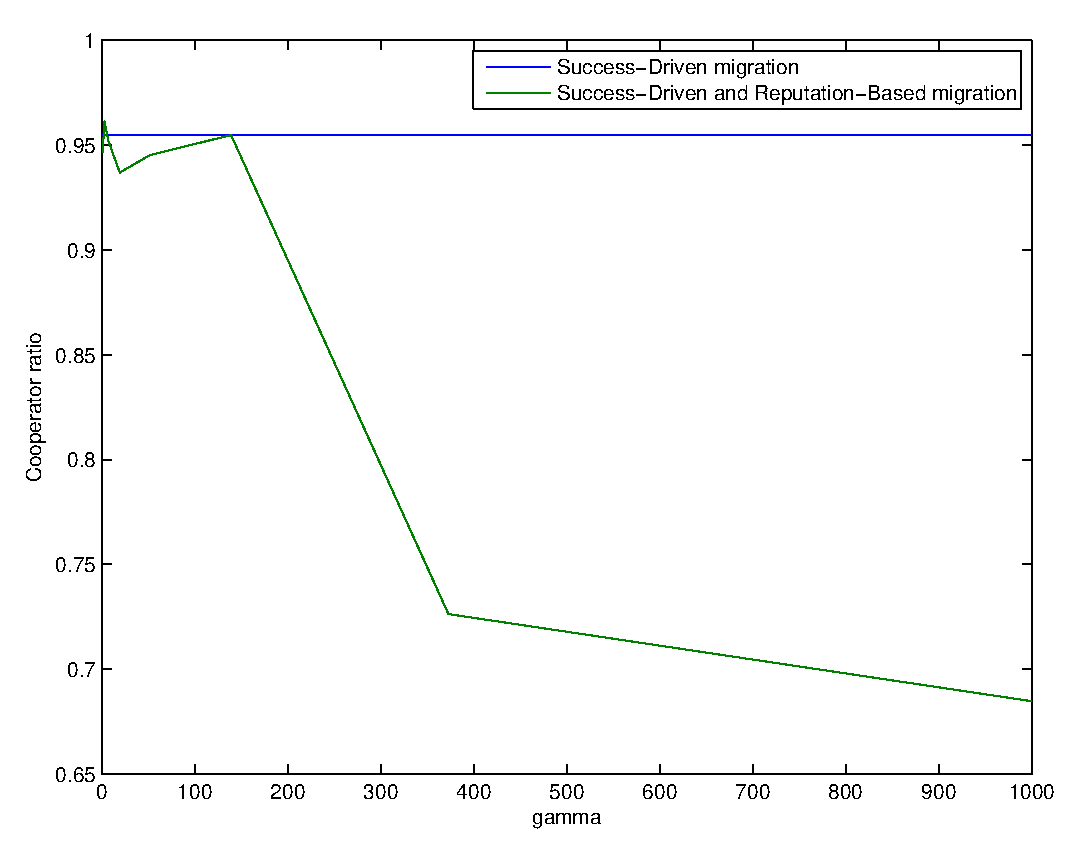
\includegraphics[width=\textwidth]{../../other/plots/alpha095.eps}
	\caption{$\alpha = 0.95$}
	\label{fig:cooperator_ratios_5000-3}
    	\end{subfigure}

	\caption{Cooperator ratios after 5000 iterations for different $\alpha$ and $\gamma$ parameters}
	\label{fig:cooperator_ratios_5000}
\end{figure}

In figure~\ref{fig:cooperator_ratios_5000}, we see that, most of the time, our model has a slightly lower cooperator ratio than the success-driven migration model.
We can see that for an $\alpha$ of $0.95$, the cooperator ratio decreases a lot for $\gamma$ over $200$. This is because with these parameters, the probability of a player to leave decreases a lot (See figure~\ref{fig:reputationeq}, reputation gets big and the divisor gets bigger) and the model gets similar to the one with imitation only.
For all other values, these parameters have no big impact on the cooperator ratios.

\begin{figure}
	\centering
        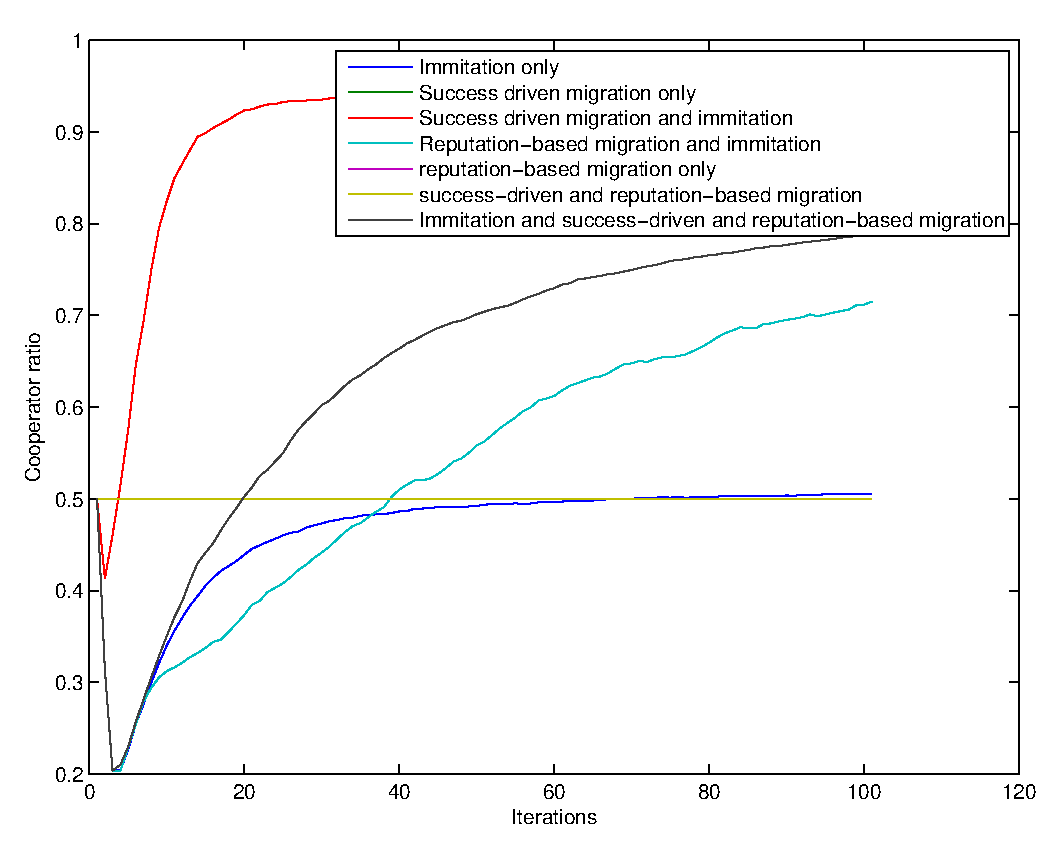
\includegraphics[width=0.5\textwidth]{../../other/plots/cooperator-ratio-evolution.eps}
	\caption{The first 100 iterations of a simulation. $\alpha = 0.5$ and $\gamma = 300$.}
	\label{fig:ratio_drop}
\end{figure}

In figure~\ref{fig:ratio_drop}, you can notice a drop in cooperator ratio at the beginning of the simulation for all the models which implement the imitation. This happened in all our simulations. The big rate of migration of the success-driven migrations compensate part of this drop.

\newpage
\subsection{Patterns}

In this part, we will look at how cooperators and defectors place themselves on the grid. We printed the grid for each model after a fixed number of iterations. We put a blue point where there was a cooperator, a red point where there was a defector and let a white space for each empty space.

\begin{figure}[H]
	\centering
	\begin{subfigure}[t]{0.3\textwidth}
        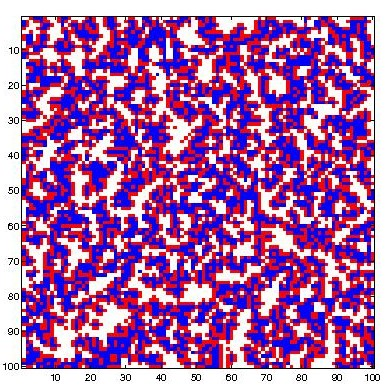
\includegraphics[width=\textwidth]{../../other/grids/m1-t200-a5-g300.jpg}
	\caption{Success-Driven migration}
	\label{fig:grids_no_imitation1}
    	\end{subfigure}
	\begin{subfigure}[t]{0.3\textwidth}
        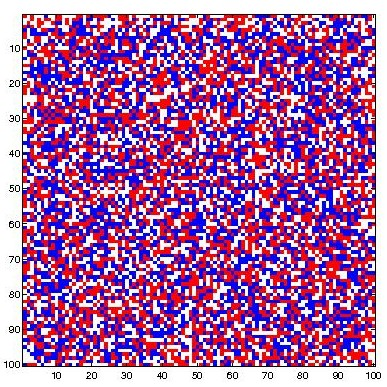
\includegraphics[width=\textwidth]{../../other/grids/m4-t200-a5-g300.jpg}
	\caption{Reputation-Based migration}
	\label{fig:grids_no_imitation4}
    	\end{subfigure}
	\begin{subfigure}[t]{0.3\textwidth}
        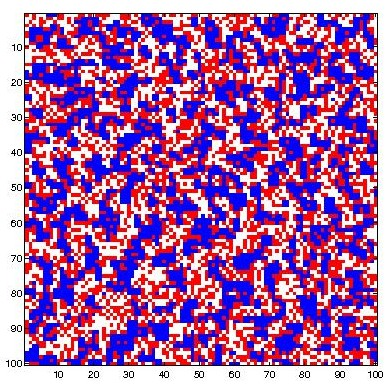
\includegraphics[width=\textwidth]{../../other/grids/m5-t200-a5-g300.jpg}
	\caption{Success-Driven and Reputation-Based migration}
	\label{fig:grids_no_imitation5}
    	\end{subfigure}

	\caption{Grids after 200 iterations for the models without imitation. We used the parameters $\alpha = 0.5$ and $\gamma = 300$.}
	\label{fig:grids_no_imitation}
\end{figure}

Figure~\ref{fig:grids_no_imitation} shows the patterns of the cooperators and defectors for the three models without imitation. In these models, the cooperator ratio stays fix at $50\%$. The first thing that we can see is that in our model (\ref{fig:grids_no_imitation5}) and the success-driven migration model (\ref{fig:grids_no_imitation1}), the cooperators arrange themselves in clusters whereas they are randomly placed in the reputation-based migration model (\ref{fig:grids_no_imitation4}).
This randomness in the reputation-based migration model is again due to the players being placed randomly on the grid when they migrate.
In the two other models, the players choose where they go based on their interest and thus the cooperators go near other cooperators because they give them the best payoff.

If we compare the success-driven migration model and our model, the main difference is in the patterns of the defectors. In the success-driven migration, the defectors are almost all placed around a cooperator cluster whereas in our model they are randomly placed on the grid. This difference can be explained by the fact that in our model, the players migrate only when their neighbours have a worse reputation than them. Since the defectors have a bad reputation, they generally don't move and stay at the random place they were assigned at the beginning. In the success-driven migration model, the defectors migrate and go around cooperators since they give them the best payoff.


\begin{figure}[H]
	\centering
	\begin{subfigure}[t]{0.26\textwidth}
        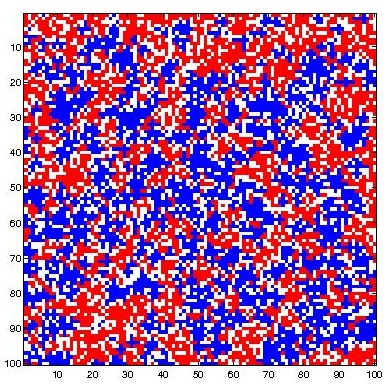
\includegraphics[width=\textwidth]{../../other/grids/m0-t200-a5-g300.jpg}
	\caption{Imitation only}
	\label{fig:grids_imitation0}
    	\end{subfigure}
	\begin{subfigure}[t]{0.26\textwidth}
        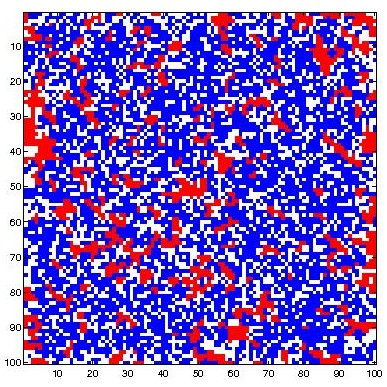
\includegraphics[width=\textwidth]{../../other/grids/m3-t200-a5-g300.jpg}
	\caption{Reputation-Based migration}
	\label{fig:grids_imitation3}
    	\end{subfigure}

	\begin{subfigure}[t]{0.26\textwidth}
        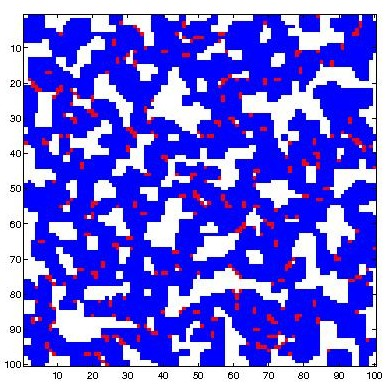
\includegraphics[width=\textwidth]{../../other/grids/m2-t200-a5-g300.jpg}
	\caption{Success-Driven migration}
	\label{fig:grids_imitation2}
    	\end{subfigure}
	\begin{subfigure}[t]{0.26\textwidth}
        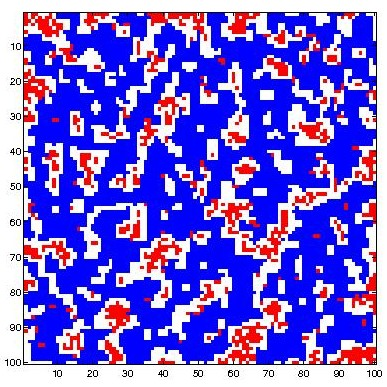
\includegraphics[width=\textwidth]{../../other/grids/m6-t200-a5-g300.jpg}
	\caption{Success-Driven and Reputation-Based migration}
	\label{fig:grids_imitation6}
    	\end{subfigure}

	\caption{Grids after 200 iterations for the models with imitation. We used the parameters $\alpha = 0.5$ and $\gamma = 300$.}
	\label{fig:grids_imitation}
\end{figure}

Figure~\ref{fig:grids_imitation} shows the patterns of cooperators and defectors in the models with imitation. We can see the same two effects previously analysed for the models without imitation, but in different forms.
The randomness of placement in the reputation-based migration model (\ref{fig:grids_imitation3}) induces a grid where the players are randomly placed on the grid and the empty space is randomly spread on the grid. In the success-driven migration model (\ref{fig:grids_imitation2}) and our model (\ref{fig:grids_imitation6}), the cooperators are organized in denser clusters because this is where they get the biggest payoff.
This time, the difference between the success-driven migration model and our model is that in our model, the defectors are isolated. This is again because the defectors have little tendency to migrate in our model and the cooperator go away from them.

\subsection{Discussion}

All the three last points showed us that the combination of success-driven migration and reputation-based migration gives indeed in the results a combination of the two.

One of the drawback of the reputation-based migration model was its randomness and unpredictability. Our model gives stability to this reputation-based migration by adding the choice of the place to migrate. In terms of convergence, cooperator ratios and cooperator patterns, our model distinguish itself from the reputation-based migration model by getting the predictability of the success-driven migration model.

Our model doesn't get cooperator ratios as high as the success-driven migration model. However, it gets ratios higher than 90\% with almost all the parameters $\alpha$ and $\gamma$ we tested. This is higher than the reputation-based migration model.

Finally, our model manages to get this high ratio, almost as high as the one from the success-driven migration model, with a more natural way of migrating. Our model lets the player migrate based on their choice and we can see this in a slower rate of convergence. Even if the highest cooperator ratio needs more time to be reached, the cooperator still take over the defectors.


\section{Summary and Outlook}

We used MATLAB to implement the prisoner's dilemma game with imitation and with three different migration models :
\begin{enumerate}
	\item Success-Driven migration
	\item Reputation-Based migration
	\item Success-Driven and Reputation-Based migration (our model)
\end{enumerate}
We ran simulations of the game for the three different models and compared the results. The purpose was to find if our model, which is a more natural one based on choice instead of randomness, can have a cooperator ratio higher than or as high as the other models.

Our model was found to converge rapidly to a high ratio of cooperators. This convergence in thousands of iterations was similar to the one of the success-driven migration model but a little slower. It distinguished our model from the reputation-based migration model which didn't reach any stable state before tens of thousand of iteration.

The cooperator ratios our model converges to are almost as high as the one from the success-driven migration model but generally lower. They are still always above 90\% except for some extreme parameters. It again distinguished our model from the reputation-based migration model which tendency was to have a ratio falling to 0\%.

We didn't analyse our model under noisy conditions and an interesting next step would be to try and compare our model similarly to the work of Helbing and Yu in The outbreak of cooperation among success-driven individuals under noisy conditions [1]. Another interesting addition would be to try our model with different payoff parameters or temptation to defect.




\section{References}

\begin{enumerate}
\item Helbing, D., \& Yu, W. (2009). The outbreak of cooperation among success-driven individuals under noisy conditions. \textit{Proceedings of the National Academy of Sciences, 106}(10), 3680-3685.
\item Helbing, D., Yu, W., \& Rauhut, H. (2011). Self-organization and emergence in social systems: Modeling the coevolution of social environments and cooperative behavior. \textit{The Journal of Mathematical Sociology, 35}(1-3), 177-208.
\item Cong, R., Wu, B., Qiu, Y., \& Wang, L. (2012). Evolution of cooperation driven by reputation-based migration. \textit{PloS one, 7}(5), e35776.
\end{enumerate}









\end{document}  



 
